%%%%%%%%%%%%%%%%%%%%%%%%%%%%%%%%%%%%%%%%%
% a0poster Portrait Poster
% LaTeX Template
% Version 1.0 (22/06/13)
%
% The a0poster class was created by:
% Gerlinde Kettl and Matthias Weiser (tex@kettl.de)
% 
% This template has been downloaded from:
% http://www.LaTeXTemplates.com
%
% License:
% CC BY-NC-SA 3.0 (http://creativecommons.org/licenses/by-nc-sa/3.0/)
%
%%%%%%%%%%%%%%%%%%%%%%%%%%%%%%%%%%%%%%%%%

%----------------------------------------------------------------------------------------
%	PACKAGES AND OTHER DOCUMENT CONFIGURATIONS
%----------------------------------------------------------------------------------------

\documentclass[a0,portrait]{a0poster}

\usepackage[portuguese]{babel}%Formata as entradas para PT-BR
\usepackage[utf8]{inputenc}
%\usepackage{verbatim}
\usepackage[document]{ragged2e}
\usepackage{multicol} % This is so we can have multiple columns of text side-by-side
\columnsep=100pt % This is the amount of white space between the columns in the poster
\columnseprule=3pt % This is the thickness of the black line between the columns in the poster

\usepackage[svgnames]{xcolor} % Specify colors by their 'svgnames', for a full list of all colors available see here: http://www.latextemplates.com/svgnames-colors

\usepackage{times} % Use the times font
%\usepackage{palatino} % Uncomment to use the Palatino font
%\usepackage{varioref}
%\usepackage{hyperref}
%\usepackage{epsfig}
\usepackage{graphicx} % Required for including images
\graphicspath{{figures/}} % Location of the graphics files
\usepackage{booktabs} % Top and bottom rules for table
\usepackage[font=small,labelfont=bf]{caption} % Required for specifying captions to tables and figures
\usepackage{amsfonts, amsmath, amsthm, amssymb} % For math fonts, symbols and environments
\usepackage{mathrsfs}
\usepackage{wrapfig} % Allows wrapping text around tables and figures
\usepackage{setspace}
\usepackage[english, ruled, linesnumbered]{algorithm2e}
\usepackage{algorithmic}
\theoremstyle{plain}
\newtheorem{teorema2}{Teorema}[]

\theoremstyle{definition}
\newtheorem{definicao}{Definição}[]

\begin{document}
\onehalfspacing
%----------------------------------------------------------------------------------------
%	POSTER HEADER 
%----------------------------------------------------------------------------------------

% The header is divided into two boxes:
% The first is 75% wide and houses the title, subtitle, names, university/organization and contact information
% The second is 25% wide and houses a logo for your university/organization or a photo of you
% The widths of these boxes can be easily edited to accommodate your content as you see fit

\begin{center}
\vspace*{-3.8cm}
    
\includegraphics[width=0.18\textwidth]{logo} 
	\hspace{55.5cm}
	
\includegraphics[width=0.1\textwidth]{vertical_extenso_fundo_claro_ok.png} 
	%\hspace{3.5cm}
	%
\includegraphics[width=0.1\textwidth]{cnpq}
\vspace{1,5cm}
\end{center}

\vspace{-10.5cm}
\begin{minipage}[b]{1.0\linewidth} %default 0.75
\begin{center}
\Huge \textbf{\textsc{Localização de Sensores e Geometria de Distâncias}}\\
%\Huge \textbf{T\'ITULO (EM MAI\'UšSCULO)}\\% Title
%\Huge\textit{An Exploration of Complexity}\\[2cm] % Subtitle
\vspace{0.3cm}\huge \textbf{Guilherme Philippi$^{1}$, Felipe Fidalgo$^{2}$}\\
%\huge \textbf{}\\
[0.5cm] % Author(s)
\huge Universidade Federal de Santa Catarina\\[0.4cm] % University/organization
\Large \texttt{g.philippi@grad.ufsc.br$^{1}$, felipe.fidalgo@ufsc.br$^{2}$}\\
\end{center}
\end{minipage}
%
\vspace{1cm} % A bit of extra whitespace between the header and poster content


%----------------------------------------------------------------------------------------

\begin{multicols}{2} % This is how many columns your poster will be broken into, a portrait poster is generally split into 2 columns

\justify % Justify all text

%----------------------------------------------------------------------------------------
%	Introdu\c c\~ao
%----------------------------------------------------------------------------------------

%\begin{abstract}
\section*{Motivação}
\vspace{-1cm}
Percebe-se uma tendência de mercado na adoção de sistemas autônomos móveis como solução para diversos problemas de engenharia, como o controle do estoque em um armazém, sistemas de logística, de transporte ou o cultivo de grandes áreas de plantio. A maior motivação deste trabalho decorre de que, seja o sistema autônomo ou não, o controle desses objetos se dá a partir da obtenção de suas localizações e por vezes tais objetos estão limitados a medir distâncias \cite{savvides2001dynamic}. Isto é, tem-se um problema inverso, onde deseja-se calcular localizações através dos dados de distâncias.
\vspace{-1cm}
\section*{Geometria de Distâncias}\vspace{-0.7cm}
A \textit{Geometria de Distâncias}, termo cunhado por Leonard Blumenthal em 1953, se preocupa com os aspectos geométricos da disposição de objetos em determinado espaço métrico. Blumenthal se baseou nos trabalhos de Arthur Cayley que, em 1841, generalizou a fórmula de Herão (que relaciona a área de um triângulo com dados de distâncias) através da construção de um determinante que calcula o conteúdo (volume $n$-dimensional) de um $k$-simplex, tema que fora reestudado por Karl Menger em 1928, trabalhando numa construção axiomática da geometria através de distâncias. Blumenthal acreditava que o problema mais importante nesta área era o \textit{Problema de Subconjunto}, que consistia em encontrar condições necessárias e suficientes a fim de decidir quando uma matriz simétrica era uma \textit{Matriz de Distâncias}. A restrição desse problema à métrica euclidiana chama-se \textit{Problema de Matrizes de Distâncias Euclidianas}, que foi flexibilizado por Yemini em 1979 ao considerar um conjunto de distâncias esparso, o que possibilitou a reformulação do problema fundamental utilizando Teoria de Grafos \cite{carlileGDandAplications}.

\begin{definicao}[Problema de Geometria de Distâncias, ou DGP]
	Dados um grafo simples, ponderado e conectado $G = (V, E, d)$ e um inteiro $K>0$, encontre uma realização $x: V \longrightarrow \mathbb{R}^K$ tal que:
	\begin{equation}
		\forall \{u,v\} \in E, \hspace{0.5cm} \lVert x(u) - x(v) \rVert = d(u,v). \label{eq:DGP}
	\end{equation}
\end{definicao}

\noindent Diversas aplicações do DGP surgiram na literatura, induzindo novos subproblemas. Um estudo taxonômico deles foi realizado por Liberti \textit{et. al.} em \cite{carlileGDandAplications} e a aplicação que aqui nos interessa é conhecido como \textit{Wireless Sensor Network Localization} (WSNL).
\vspace{-1cm}
\section*{Localização de Sensores}
\vspace{-0.7cm}
\begin{definicao}[Problema WSNL]
	Obter solução única do DGP com $K= 2$ ou $3$, onde são fornecidos os \textit{Vértices Âncoras} $A\subset V$ que já possuem uma posição em $\mathbb{R}^k$ conhecida.\label{def:wsnl}
\end{definicao}

\noindent A unicidade está relacionada com a rigidez do grafo que define o problema \cite{eren2004rigidity}. A \textit{trilateração} é um método para solucionar um WSNL definido por um $(K+2)$-clique onde $(K+1)$ vértices são âncoras \cite{libertiEDG}. Nele, a solução do problema restringe-se a resolver um sistema linear do tipo $Ay = b$, \textit{i.e.}, se $A$ não é singular, a posição do $(K+2)$-ésimo vértice é obtido calculando-se $y = A^{-1}b = x_{K+2}$. No geral, a singularidade de $A$ está relacionada com a existência de vértices com posições coincidentes. Portanto, dado um $(K+2)$-clique, sabe-se que se ele possuir uma realização em $\mathbb{R}^K$ e não possuir vértices coincidentes, ela é única a menos de rotações e translações. Com isso, pode-se utilizar a trilateração de forma iterativa para realizar de forma única um grafo completo e, além disso, estende-se esse resultado com o objetivo de aplicar a trilateração em grafos ``completos por partes'' ao definir uma ordenação conveniente nos vértices do grafo.

\begin{definicao}[Ordem de $K$-Lateração]
	Se $<$ é uma ordem em $V$ e $v\in V$ é um vértice qualquer, então $\gamma(v) = \{u\in V \;|\; u<v \}$ é dito conjunto de antecessores de $v$ em relação a $<$, $N_G(v)$ é o conjunto de vértices adjacentes a $v$ em $G$ e $\rho(v) = |\gamma(v)|+1$ é dito posto de $v$ em $<$. Dado um grafo $G=(V,E)$, uma ordenação $<$ sobre $V$ é chamada \textit{Ordem de $K$-Lateração} se:
	
	\begin{enumerate}
		\vspace{-0.2cm}
		\item os primeiros $K+1$ vértices de $<$ induzem um $(K+1)$-clique $G_o$ em $G$;
		\vspace{-0.2cm}
		\item todo vértice $v$, com $\rho(v) > K+1$, tem $\lvert N_G(v) \bigcap \gamma(v)\rvert \geq K+1$.
	\end{enumerate}
\end{definicao}

\noindent Um grafo $G = (V,E)$ é dito \textit{$K$-Laterativo} se há uma ordem de $K$-lateração sobre $V$ e não há vértices coincidentes. Como a existência de uma ordem de $K$-lateração garante que sempre haverá ao menos $K+1$ vértices já realizados antecessores a todo vértice $v \in V$, com $\rho(v) > K+1$, será possível aplicar a trilateração a todo vértice, viabilizando o seguinte resultado:

\begin{teorema2}
	Se um grafo $K$-laterativo em $\mathbb{R}^K$ possuir realização, ela é única.
\end{teorema2}

\vspace{-1cm}
\section*{Simulações Computacionais}
\vspace{-0.7cm}
Assim, define-se o Algoritmo~\ref{alg:realizacaoTrilateration} para so\-lu\-cio\-nar problemas de WSNL sobre grafos $K$-laterativos em tempo polinomial \cite{libertiEDG}. A fim de se realizar simulações computacionais, implementou-se este algorítimo em C, bem como um segundo para criar exemplares artificiais do problema com coordenadas aleatórias e um conjunto limitável de arestas extras.

\vspace{0.5cm}
\begin{algorithm}[H]
	\label{alg:realizacaoTrilateration}
	\For{$i\in \{K+2,\dots,n\}$}{
		sejam $U \subset \lvert N_G(v) \bigcap \gamma(v)\rvert$, com $\lvert U\rvert = K+1$, e $W = \{x_j\ |\ j\in U\}$\;
		$x_i \gets$ Trilateracao$(W)$\;
		\For{$\{j\in \{(N_G(v) \bigcap \gamma(v)) \setminus U\} \ ; \ j<i\}$}{
			\If{$\lVert x_i - x_j\rVert \ne d_{ij}$}{
				$x_i = \emptyset$\;
				\textbf{break}\;
			}
		} 
		\If{$x_i = \emptyset$}{
			\textbf{return} $\emptyset$\;
		}
	}
	\textbf{return} $x$\;
	\caption{$x =$ RealizacaoIterativa$(G,d, K, x)$, adaptado de \cite{libertiEDG}}
\end{algorithm}
\vspace{0.5cm}

\noindent Com isso, para exemplares de $n$ vértices e com $1\%$ de arestas extras, a Figura 1 mostra o tempo decorrido para cada realização. Como utiliza-se vértices já realizados para realizar novos, acumula-se erros no processo. Podemos calcular esses erros com o chamado \textit{mean distance error}.

\begin{definicao}[\textit{Mean Distance Error}, ou MDE]
	Seja $G= (V,E,d)$ um grafo ponderado que define uma instância DGP. Se $\{x_1, \dots, x_n\}$ é um conjunto que define uma realização dos $n$ vértices de $G$ então,
	$MDE(x) = \frac{1}{|d\;|} \sum_{i,j}^{}\frac{|||x_i - x_j|| - d_{i,j}|}{d_{i,j}} .$
\end{definicao}

\vspace{0.5cm}
\begin{minipage}[b]{1.0\linewidth}\label{fig:resultados}
	\begin{center}
		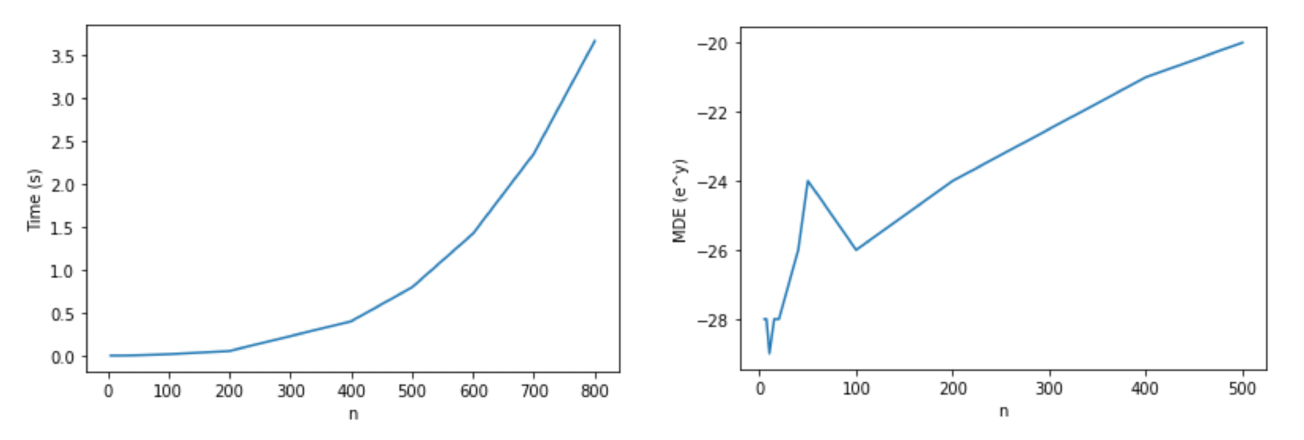
\includegraphics[width=37cm]{resu.png}
		\captionof{figure}{A esquerda o tempo de processo e, a direita, a ordem de grandeza associada ao MDE das soluções.}
	\end{center}
\end{minipage}
\vspace{-1cm}

\noindent Observe que há uma linearização no gráfico que representa o MDE da solução, pois este cresceu exponencialmente e variou sua ordem de grandeza entre $10^{-28}$ a $10^{-20}$ de 5 a 500 vértices. Esse comportamento se deu por conta dos erros acumulados entre as iterações. Também, o tempo de processamento cresceu polinomialmente, conforme o proposto.

\vspace{-1cm}
\begin{thebibliography}{00}
	\vspace{-0.7cm}
	\bibitem{savvides2001dynamic} Savvides, A., Han, C. C., e Strivastava, M. B. Dynamic fine-grained localization in ad-hoc networks of sensors.\textit{ In Proceedings of the 7th annual international conference on Mobile computing and networking}, 166-179. DOI: 10.1145/381677.381693
	
	\bibitem{carlileGDandAplications} Liberti, L., Lavor, C., Maculan, N., e Mucherino, A. (2014). Euclidean distance geometry and applications. \textit{SIAM review}, 56:3-69. DOI:10.1137/120875909
	
	\bibitem{eren2004rigidity} Eren, T., Goldenberg, O. K., Whiteley, W., Yang, Y. R., Morse, A. S., Anderson, B. D., e Belhumeur, P. N. Rigidity, computation, and randomization in network localization. \textit{IEEE INFOCOM} 2004 volume 4, pp. 2673-2684. DOI: 10.1109/INFCOM.2004.1354686
	
	
	
	\bibitem{libertiEDG} Liberti, L.; Lavor, C. \textit{Euclidean Distance Geometry}. Springer, Berlin, 2017.
	
	
	
\end{thebibliography}

\vspace{-1cm}
\section*{Agradecimentos}\vspace{-0.7cm}
Este trabalho foi realizado com o apoio do Conselho Nacional de Desenvolvimento	Científico e Tecnológico -- CNPq -- Brasil. Agradecemos a organização do evento e a UFSC.



%----------------------------------------------------------------------------------------

\end{multicols}
\end{document}